\documentclass[numbers=noendperiod]{scrartcl}
%Font encoding packages:
\usepackage[utf8]{luainputenc}
\usepackage[T1]{fontenc}
\usepackage[ngerman]{babel}
\usepackage[a4paper,margin=0.75in, bottom=1in]{geometry}
%Extension packages:
\usepackage{listings}
\usepackage{mdframed}
\usepackage[kpsewhich]{minted}
\usepackage{courier}
\usepackage{amsmath}
\usepackage{amssymb}
\usepackage{wasysym}
\usepackage{enumerate}
\usepackage{graphicx}

\begin{document}
	
\definecolor{bg}{RGB}{230,230,230}
	
\hrulefill
\begin{center}
	\bfseries % Fettdruck einschalten
	\sffamily % Serifenlose Schrift
	\begin{huge}
		ALPIV: Nichtsequentielle und verteilte Programmierung
	\end{huge}\\
	\begin{Large}
		Sommersemester 2017, 5. Übungsblatt
	\end{Large}\\
	\begin{small}
		Philipp Thiele, Luis Herrmann; Tutor: Alexander Kauer; Fr 12:00-14:00
	\end{small}
	
	\vspace{-10pt}
\end{center}
\hrulefill

\definecolor{bg}{RGB}{230,230,230}
\newcommand{\inputmintedframed}[2]{
	\begin{mdframed}[linecolor=bg,backgroundcolor=bg]
		\inputminted[mathescape,breaklines,linenos,numbersep=5pt,tabsize=3]{#1}{#2}
\end{mdframed}}

\section*{1. Aufgabe}
	\begin{enumerate}
		\item $\Box A \land \Diamond B \Rightarrow \Diamond (A \land B)$ ist eine wahre Aussage. Beweis:
		\begin{align}
			\Box A \land \Diamond B \Leftrightarrow &(\forall j \ge i : A \text{ in } S_j) \land (\exists k\ge i : B \text{ in } S_K)\\
			\Leftrightarrow &\exists k \ge i \forall j\ge i: A \text{ in } S_j \land B \text{ in } S_k\\
			\Rightarrow & \exists k \ge i : A\text{ in } S_k \land B \text{ in } S_k\\
			\Leftrightarrow & \exists k \ge i : (A \land B) \text{ in } S_k \Leftrightarrow \Diamond (A\land B)
		\end{align}
		
		\item $\Box (A \lor B) \Rightarrow (\Box A \lor \Diamond B)$ ist wahre Aussage. Beweis durch Kontraposition:
		\begin{align}
			\lnot (\Box A \lor \Diamond B) \Rightarrow & (\lnot \Box A ) \land (\lnot \Diamond B)\\
			\Leftrightarrow &(\Diamond \lnot A) \land (\Box \lnot B)\\
			\overset{1.}{\Rightarrow} &\Diamond(\lnot A \land \lnot B)\\
			\Rightarrow & \Diamond\lnot (A \lor B) \Leftrightarrow \lnot \Box (A \lor B)
		\end{align}
		
		\item $\Diamond A \land \Diamond B \Rightarrow \Diamond (A \land B)$ ist falsch.
		In Quatorensprache ausgeführt:
		\begin{align}
			&\Diamond A \land \Diamond B \Leftrightarrow (\exists j \ge i : A \text{ in } S_j) \land (\exists k \ge i : B \text{ in } S_k) \Leftrightarrow \exists j \ge i \exists k \ge i : A \text{ in } S_j \land B \text{ in } S_k\\
			&\Diamond (A \land B) \Leftrightarrow \exists j\ge i : A \land B \text{ in } S_j \Leftrightarrow \exists j\ge i \exists k \ge i : A \text{ in } S_j \land B \text{ in } S_k \land j = k\\
			&\Leftrightarrow (\exists j \ge i : A \text{ in } S_j) \land (\exists k \ge i : B \text{ in } S_k) \land j = k
		\end{align}
		
		Offensichtlich folgt aus der linken Seite der Implikation noch nicht, dass das $j = k$, also sind beide Aussage nicht äquivalent. Betrachte folgendes Gegenbeispiel. Sei $(S_i)_{i\in \mathbb{N}}$ eine Sequenz von Zuständen und
		\begin{align}
			&A(S_i) ) := \begin{cases}
			true, &i=1\\
			false, &\text{sonst}
			\end{cases}
			&& B(S_i) := \begin{cases}
			true, &i=2\\
			flase, &\text{sonst}
			\end{cases}
		\end{align}
		Offenbar gilt $\Diamond A \land \Diamond B$, aber es gelten nie $A \land B$ gleichzeitig, also $\Diamond (A\land B) \equiv false$.
		
	\end{enumerate}


\section*{2. Aufgabe}
	Wir konstruieren die folgenden Szenarien:
	
	Szenario 1: $n=4$, $k=2$\\
	\begin{tabular}{|c|c|c|}
		Ausgeführter Thread & Ausgeführte Programmzeilen & Endzustand Variablen\\\hline
		Thread1:& p2,3,4,5& (count: 1, temp: 1, S: 1, D: 0)\\
		Thread2:& p2,3,4,5& (count: 0, temp: 0, S: 1, D: 0)\\
		Thread3:& p2,3,4,5& (count: -1, temp: -1, S: 1, D: 0)\\
		Thread4:& p2,3,4,5& (count: -2, temp: -2, S: 1, D: 0)\\
		Thread1:& p6,9,10,11,12,13& (count: -1, temp: 1, S: 1, D: 1)\\
		Thread2:& p6,9,10,11,12,13& (count: 0, temp: 0, S: 1, D: 2)\\
	\end{tabular}
	
	Szenario 2: $n=3$, $k=2$\\
	\begin{tabular}{|c|c|c|}
		Ausgeführter Thread & Ausgeführte Programmzeilen & Endzustand Variablen\\\hline
		Thread1:& p2,3,4,5& (count: 1, temp: 1, S: 1, D: 0)\\
		Thread2:& p2,3,4,5& (count: 0, temp: 0, S: 1, D: 0)\\
		Thread3:& p2,3,4,5& (count: -1, temp: -1, S: 1, D: 0)\\
		Thread1:& p6,9,10,11,12,13& (count: 0, temp: 1, S: 1, D: 1)\\
		Thread1:& p2,3,4,5& (count: -1, temp: -1, S: 1, D: 1)\\
		Thread2:& p6,9,10,11,12,13& (count: 0, temp: 0, S: 1, D: 2)\\
	\end{tabular}\\

	Lokale Variablen beziehen sich immer auf den zuletzt ausgeführten Thread.

\section*{3. Aufgabe}
	\inputmintedframed{java}{Wasser.java}
	
	Da beim Eintritt in die kritische Sektion sowohl der Lock für Wasserstoff- als auch für Sauerstoffatome acquired wird, können nie mehrere Atome gleichzeitig die globalen Variablen manipulieren (oder vergleichen). Dabei wird durch die Erzeugung der ReentrantLocks mit Übergabe des Parameters \text{true} eine FIFO-Warteschlange für die Threads gebildet, welche die entsprechenden Locks aufnehmen. Wenn ein Atom auf die imaginäre "Membran" trifft, wird (je nach Atom) die globale Anzahl der Wasserstoff- bzw. Sauerstoffatome an der Membran (\textit{hCounter} bzw. \textit{oCounter}) hochgezählt und es wird überprüft, ob die aktuell vorhandenn Atome reichen, um ein H2O-Molekül zu bilden. Ist das der Fall, so wird sofort ein H2O-Molekül "gebildet" indem die Anzahl der Atome an der Membran entsprechend reduziert wird und die anderen zwei zur Bildung des Moleküls benötigten Atome werden "geweckt".
	
	Aufgrund der FIFO-Warteschlange kann es nicht passieren, dass ein gerade in die Membran eintretendes Atom die austretenden Atome überholt, da die Zählvariablen unter gegenseitigem Ausschluss manipuliert und verglichen werden und ferner die FIFO-Warteschlange garantiert, dass soeben "aufgeweckte" Atome vor neu eintreffenden abgearbeitet werden.\\
	
	Offensichtlich gilt die Invariante:
	\begin{equation}
		hCounter \le 2 \lor oCounter \le 1
	\end{equation}
	Denn sonst würde in einem Schritt kein H2O-Molekül gebildet obwohl genug Atome dafür vorhanden sind.
	
	\section*{4. Aufgabe}
	
	Wir konstruieren zunächst den Resource-Allocation-Graphen:
	
	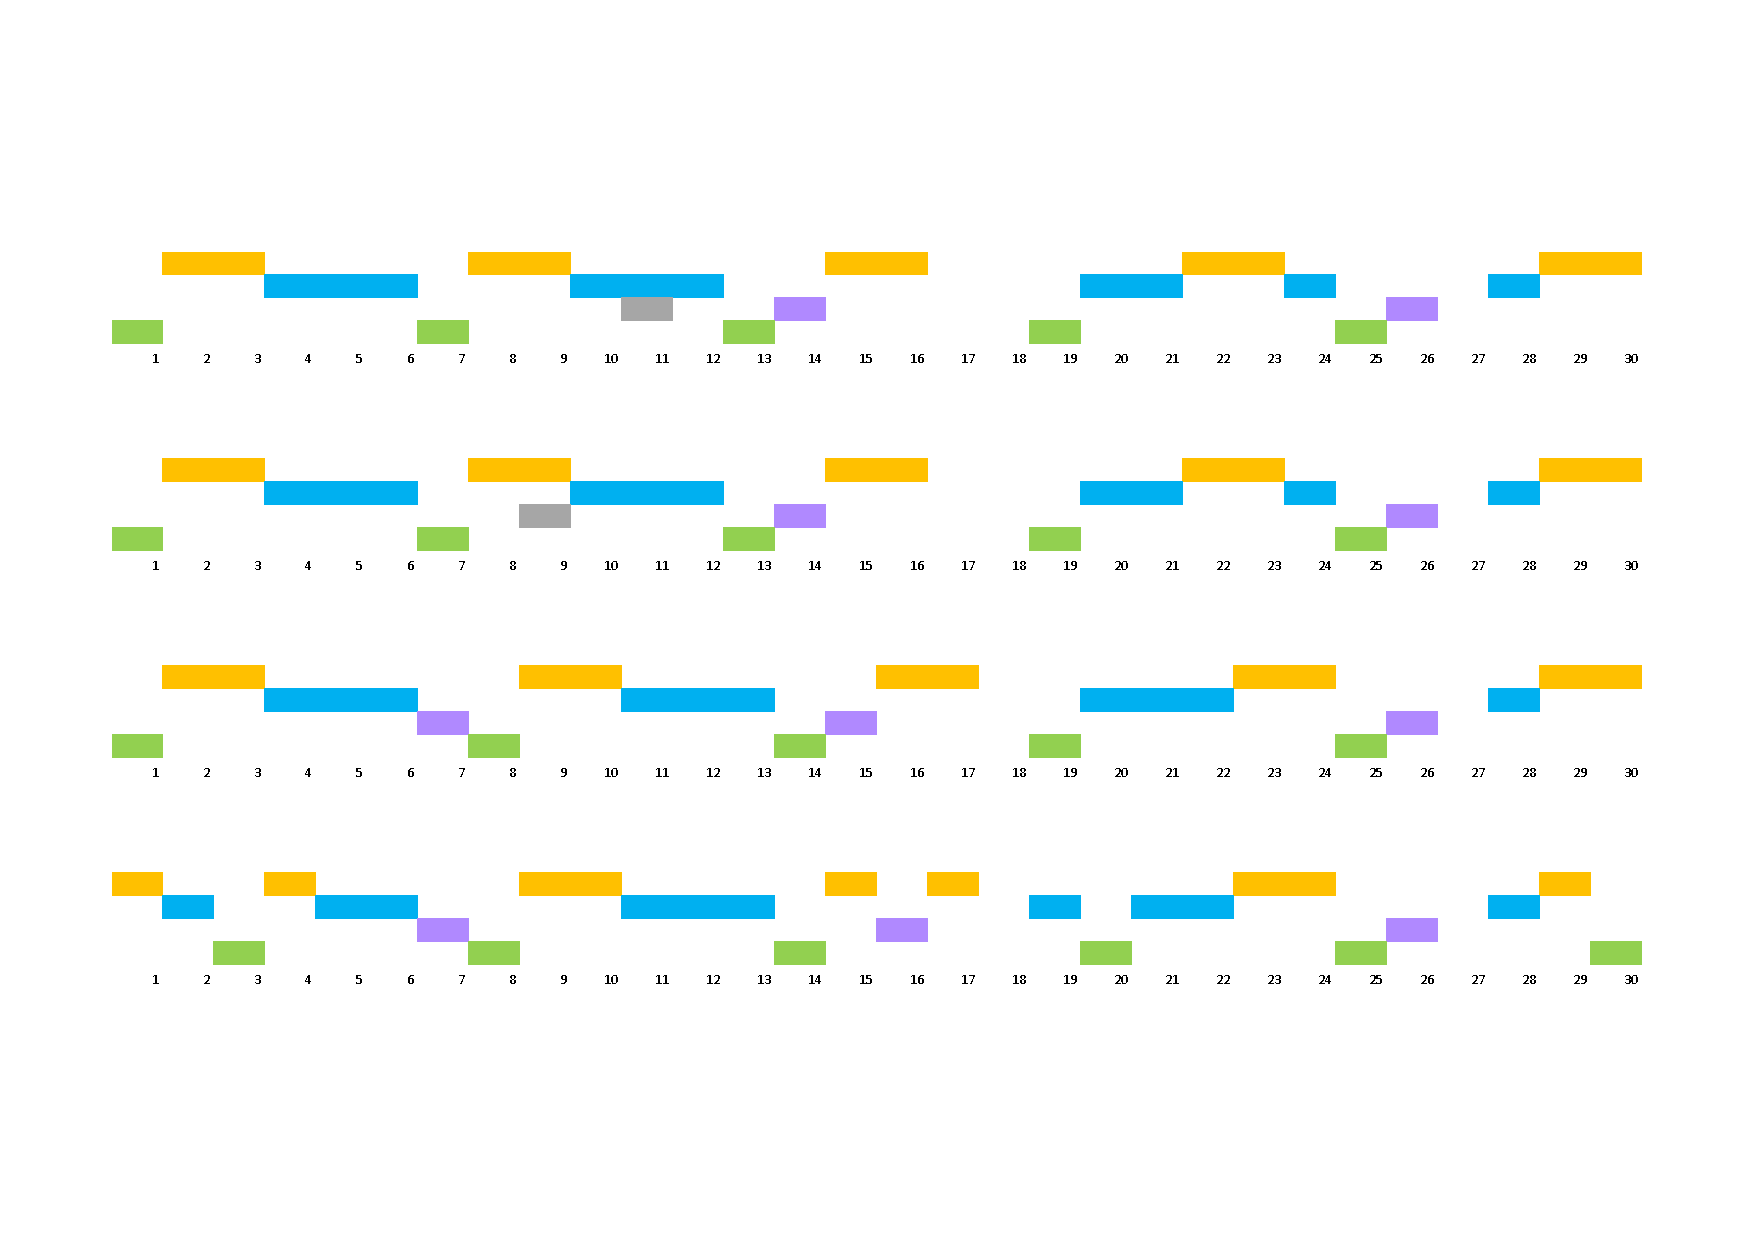
\includegraphics[width=\textwidth,page=1,trim={2 2 2 4},clip]{diagramme.pdf}
	
	
	Offenbar gibt es mehrere Zyklen:
	$T_1 \to R_3 \to T_2 \to R_2$, $T_1 \to R_3 \to T_5 \to R_4 \to T_3 \to R_2$ und $T_1 \to R_3 \to T_5 \to R_4 \to T_3 \to R_3 \to T_2 \to R_2$, allerdings taucht noch keine Verklemmung auf, denn an allen Zyklen sind $T_1, T_2, R_2$ und $R_3$ beteiligt; die Auftreten von Deadlocks hängt somit im Wesentlichen von diesen zwei Prozessen ab, aber die von den zwei diesen Threads angeforderten Ressourcen werden auch von anderen Threads belegt, die diese im nächsten Schritt freigeben können. Wird zum Beispiel im nächsten Schritt $R_2$ von $T_4$ freigegeben und $T_1$ zugewiesen, kommt es nicht zum Deadlock.
	
	Allerdings ist diese Konfiguration Deadlock-gefährdet. Nehmen wir an, $T_4$ gibt im nächsten Schritt eine Ressource von $R_3$ frei und der Scheduler gewährt $T_3$ Zugriff. Dann befindet wir uns in einem Deadlock, denn $T_1$, $T_2$ und $T_3$ warten dann untereinander auf die Freigabe von Ressourcen in $R_2$, $R_3$, und eine Ressource in $R_3$ kann auch nicht von $T_5$ freigegeben werden, da dieses auf die Freigabe von $R_4$ wartet.
	
\end{document}
